\documentclass[12pt, a4paper]{article}

\usepackage{amsmath}
\usepackage{amsfonts}
\usepackage{amssymb}
\usepackage{graphicx}
\usepackage{float}
\usepackage{listings}
\usepackage{rotating}
\usepackage{tikz}
\usepackage{verbatim}
\pdfgentounicode=1
\pdfmapline{+cyberb@Unicode@  <cyberbit.ttf}

\begin{document}

\title{BCurve}
\author{P. Baillehache}
\date{\today}
\maketitle

\tableofcontents

\section*{Introduction}

BCurve is C library to manipulate Bezier curves and surfaces of any dimension and order.\\ 

It offers function to create, clone, load, save and modify a curve, to print it, to scale, rotate (in 2D) or translate it, to get its approximate length (sum of distance between control points), to create a BCurve connecting points of a point cloud, to get the weights (coefficients of each control point given the value of the parameter of the curve), and to get the bounding box.\\ 

The library also includes a SCurve structure which is simply a GSet<BCurve> to manipulate a set of curves.\\

The library also includes a BSurf structure which is the extension of BCurve for input space dimension higher than 1.\\

\section{Definitions}

\subsection{BCurve definition}

A BCurve $B$ is defined by its dimension $D\in\mathbb{N}^*_+$, its order $O\in\mathbb{N_+}$ and its $(O+1)$ control points $\overrightarrow{C_i}\in\mathbb{R}^D$. The curve in dimension $D$ associated to the BCurve $B$ is defined by $\overrightarrow{B(t)}$:\\
\begin{equation}
\left\lbrace
\begin{array}{ll}
\overrightarrow{B(t)}=\sum_{i=0}^OW^O_i(t)\overrightarrow{C_i}&\textrm{if }t\in[0.0,1.0]\\
\overrightarrow{B(t)}=\overrightarrow{C_0}&\textrm{if }t<0.0\\
\overrightarrow{B(t)}=\overrightarrow{C_{O}}&\textrm{if }t>1.0\\
\end{array}
\right.
\end{equation}
where, if $O=0$\\
\begin{equation}
W^0_0(t)=1.0
\end{equation}
and if $O\neq 0$\\
\begin{equation}
\left\lbrace
\begin{array}{l}
W^1_0(t)=1.0-t\\
W^1_1(t)=t\\
W^i_{-1}(t)=0.0\\
W^i_j(t)=(1.0-t)W^{i-1}_j(t)+tW^{i-1}_{j-1}(t)\textrm{ for }i\in[2,O],j\in[0,i]
\end{array}
\right.
\end{equation}

\subsection{BCurve from cloud points}

Given the cloud points made of $N$ points $\overrightarrow{P_i}$, the BCurve of order $N-1$ passing through the $N$ points (in the same order $\overrightarrow{P_0}$,$\overrightarrow{P_1}$,$\overrightarrow{P_2}$,... as given in input) can be obtained as follow.\\

If $N=1$ the solution is trivial: $\overrightarrow{C_0}=\overrightarrow{P_0}$. As well, if $N=2$ the solution is trivial: $\overrightarrow{C_0}=\overrightarrow{P_0}$ and $\overrightarrow{C_1}=\overrightarrow{P_1}$.\\

If $N>2$, we need first to define the $N$ values $t_i$ corresponding to each $\overrightarrow{P_i}$ ($\overrightarrow{B(t_i)}=\overrightarrow{P_i}$). We will consider here $t_i$ such as\\
\begin{equation}
t_i=\frac{L(\overrightarrow{P_i})}{L(\overrightarrow{P_{N-1}})}
\end{equation}
where
\begin{equation}
\left\lbrace
\begin{array}{l}
L(P_0)=0.0\\
L(P_i)=\sum^i_{j=1}\left|\left|\overrightarrow{P_{j-1}P_j}\right|\right|\\
\end{array}
\right.
\end{equation}
then we can calculate the $C_i$ as follow. We have $\overrightarrow{C_0}=\overrightarrow{P_0}$ and $\overrightarrow{C_{N-1}}=\overrightarrow{P_{N-1}}$, and others $\overrightarrow{C_i}$ can be obtained by solving the linear system below for each dimension:\\
\begin{equation}
\begin{array}{c}
\left[
\begin{array}{ccc}
W^{N-1}_1(t_1)&...&W^{N-1}_{N-2}(t_1)\\
...&...&...\\
W^{N-1}_1(t_{N-2})&...&W^{N-1}_{N-2}(t_{N-2})\\
\end{array}
\right]\left[
\begin{array}{c}
C_1\\
...\\
C_{N-2}\\
\end{array}
\right]=\\
\\
\left[
\begin{array}{c}
P_1-\left(W^{N-1}_0(t_1)P_0+W^{N-1}_{N-1}(t_1)P_{N-1}\right)\\
...\\
P_{N-2}-\left(W^{N-1}_0(t_{N-2})P_0+W^{N-1}_{N-1}(t_{N-2})P_{N-1}\right)\\
\end{array}
\right]
\end{array}
\end{equation}

\subsection{BSurf definition}

A BSurf $S$ is defined by its input dimension $D_i\in\mathbb{N}^*_+$, its output dimension $D_o\in\mathbb{N}^*_+$, its order $O\in\mathbb{N_+}$ and its $(O+1)^{D_i}$ control points $\overrightarrow{C_i}\in\mathbb{R}^{D_o}$. Control points indices are ordered as follow (for an example BSurf with $D_i=3$): (0,0,0),(0,0,1),...,(0,0,O+1),(0,1,0),(0,1,1),... \\
Note that if $D_i$ is equal to 1, a BSurf is equivalent to a BCurve.\\
The function $\overrightarrow{S}():[0.0,1.0]^{D_i}\mapsto\mathbb{R}^{D_o}$ associated to the BSurf $S$ is defined by:\\
\begin{equation}
\overrightarrow{S}(\overrightarrow{u})=\overrightarrow{R_S}(\overrightarrow{0},\overrightarrow{u},0)
\end{equation}
where
\begin{equation}
\left\lbrace
\begin{array}{ll}
\overrightarrow{R_S}(\overrightarrow{c},\overrightarrow{u},d)=\overrightarrow{B_{\lbrace\overrightarrow{C}_{I(\overrightarrow{c},d)}\rbrace}}(u_d)&\textrm{if }d=D_i-1\\
\overrightarrow{R_S}(\overrightarrow{c},\overrightarrow{u},d)=\overrightarrow{B_{\lbrace\overrightarrow{R_S}(\lbrace\overrightarrow{c}\rbrace_d,\overrightarrow{u},d+1)\rbrace}}(u_d)&\textrm{if }d\ne D_i-1\\
\end{array}
\right.
\end{equation}
where $\overrightarrow{B_{\lbrace\bullet\rbrace}}$ is the BCurve of dimension $D_o$, order $O$ and control points $\bullet$. And $\lbrace\overrightarrow{C}_{I(\overrightarrow{c},d)}\rbrace$ is the set of control points of S of indices:\\
\begin{equation}
\lbrace I(\overrightarrow{c},d)\rbrace=\lbrace
\begin{array}{l}
\sum_{i\in[0,D_i-1]|i\ne d}\left(O^{(D_i-1-i)}c_i\right)+O^{(D_i-1-d)}j
\end{array}
\rbrace_{j\in[0,O]}
\end{equation}
and $\lbrace\overrightarrow{R_S}(\lbrace\overrightarrow{c}\rbrace_d,\overrightarrow{u},d')\rbrace$ is the set of intermediate control points calculated for:\\
\begin{equation}
\lbrace\overrightarrow{c}\rbrace_d=\lbrace(\overrightarrow{c_0,c_1,..,c_{d-1},j,c_{d+1},..,c_{D_i-1}})\rbrace_{j\in[0,O]}
\end{equation}

\section{Interface}

\begin{scriptsize}
\begin{ttfamily}
\verbatiminput{../bcurve.h}
\end{ttfamily}
\end{scriptsize}

\section{Code}

\begin{scriptsize}
\begin{ttfamily}
\verbatiminput{../bcurve.c}
\end{ttfamily}
\end{scriptsize}

\section{Makefile}

\begin{scriptsize}
\begin{ttfamily}
\verbatiminput{../Makefile}
\end{ttfamily}
\end{scriptsize}

\section{Usage}

\begin{scriptsize}
\begin{ttfamily}
\verbatiminput{../main.c}
\end{ttfamily}
\end{scriptsize}

Output:\\
\begin{scriptsize}
\begin{ttfamily}
\verbatiminput{../output.txt}
\end{ttfamily}
\end{scriptsize}

BCurve example:\\
\begin{center}
\begin{figure}[H]
\centering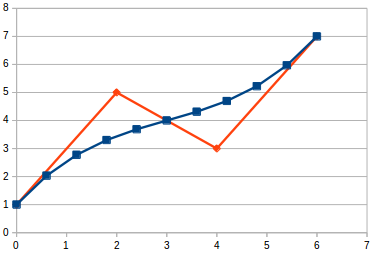
\includegraphics[width=6cm]{./res.png}\\
\end{figure}
\end{center}
BCurve transformation example:\\
\begin{center}
\begin{figure}[H]
\centering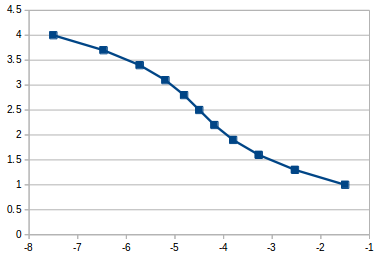
\includegraphics[width=6cm]{./resrot.png}\\
\end{figure}
\end{center}
BCurve from point cloud:\\
\begin{center}
\begin{figure}[H]
\centering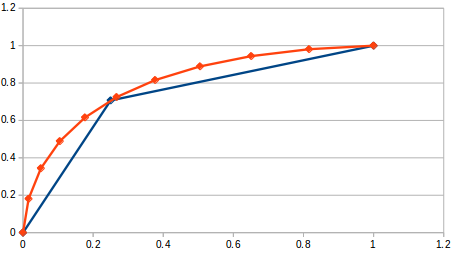
\includegraphics[width=6cm]{./cloud1.png}\\
\end{figure}
\end{center}
\begin{center}
\begin{figure}[H]
\centering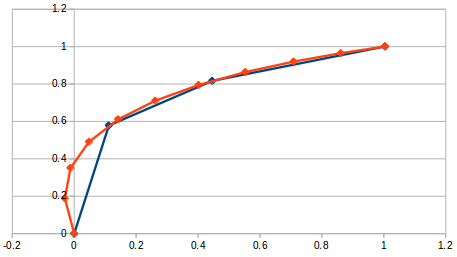
\includegraphics[width=6cm]{./cloud2.png}\\
\end{figure}
\end{center}
\begin{center}
\begin{figure}[H]
\centering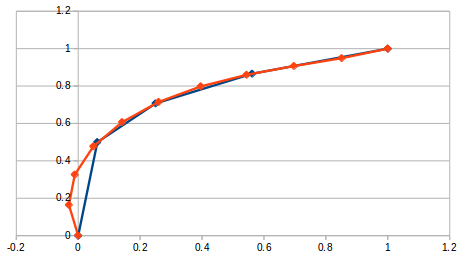
\includegraphics[width=6cm]{./cloud3.png}\\
\end{figure}
\end{center}
BSurf example:\\
\begin{center}
\begin{figure}[H]
\centering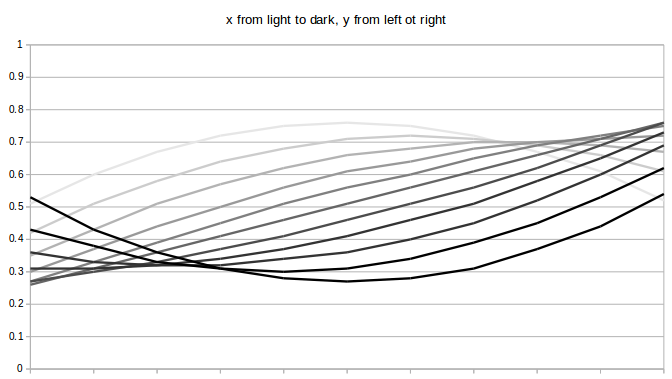
\includegraphics[width=6cm]{./bsurf.png}\\
\end{figure}
\end{center}

curve.txt:\\
\begin{scriptsize}
\begin{ttfamily}
\verbatiminput{../curve.txt}
\end{ttfamily}
\end{scriptsize}

\end{document}


